\documentclass[a4paper,10pt]{article}
\usepackage[utf8]{inputenc}
\usepackage[margin=1.5cm, bottom=2cm]{geometry}
\usepackage{fancyhdr}
\usepackage[dvipsnames]{xcolor}
\usepackage{enumitem}
\usepackage{xcolor}
\usepackage[table]{xcolor}
\usepackage{makeidx}
\usepackage[most]{tcolorbox}
\newtcolorbox{osservazioni}{
  colback=gray!8,    % sfondo grigio chiaro
  colframe=white,      % nessun bordo
  arc=2mm,            % angoli smussati
  boxrule=0pt,        % spessore bordo 0
  fontupper=\footnotesize,
  left=2mm, right=2mm, top=2mm, bottom=2mm,
  before skip=7pt,   % niente spazio prima
  after skip=15pt     % niente spazio dopo
}
\newtcolorbox{osservazioni2}{
  colback=ForestGreen!4,    % sfondo grigio chiaro
  colframe=white,      % nessun bordo
  arc=2mm,            % angoli smussati
  boxrule=0pt,        % spessore bordo 0
  fontupper=\footnotesize,
  left=2mm, right=2mm, top=2mm, bottom=2mm,
  before skip=7pt,   % niente spazio prima
  after skip=15pt     % niente spazio dopo
}
\pagestyle{fancy}
\usepackage{tikz}
\usetikzlibrary{automata, positioning}
\pagestyle{fancy}

\usepackage{makeidx}

%%%%%%%%%%%%%%%%%%%
\newcommand{\EsercitazioneNum}{12}
\newcommand{\Data}{04/12/2025}
\newcommand{\DocType}{Esercitazione} % o "Eserciziario"
\newcommand{\FullTitle}{\DocType\ \EsercitazioneNum}

\newcommand{\Header}{
\noindent
  \small \textbf{Computabilità, Complessità e Logica - a.a. 2025/26} \hfill \textbf{\FullTitle} \\[0.2cm]
  \scriptsize Matteo Liotta, \texttt{matteo.liotta@studenti.units.it} \hfill \Data \\[0.2cm]
  \noindent\makebox[\linewidth]{\rule{\linewidth}{0.4pt}} \\[0.3cm]}

\newcommand{\NewPageHeader}{
  \vfill
  \noindent\makebox[\linewidth]{\rule{\linewidth}{0.4pt}}
  \newpage
  {\Header}
}
%%%%%%%%%%%%%%%%%%%

% Numero di pagina in basso al centro
\fancyhf{}
\fancyfoot[C] \thepage
\renewcommand{\footrulewidth}{0pt} % niente linea in basso
\renewcommand{\headrulewidth}{0pt} % niente linea in alto

\begin{document}

\footnotesize  % font generale più piccolo
\Header\\[0.7cm]


%%%%%%%%%%%%%%%% FOGLIO 2

    
    %% INDEX
    \addcontentsline{toc}{section}{Esercitazione 12: \textit{Logica dei Predicati}}
    
    \noindent\Large \textbf{Esercitazione 12}: \textit{Logica dei Predicati} 
    \begin{osservazioni}
        \textbf{\textit{Nota}}. Sono indicati in \textcolor{ForestGreen}{\textit{verde}} gli esercizi a sfondo teorico, proposti per rafforzare le idee alla base dei metodi utilizzati. Sono invece indicati in \textcolor{blue}{\textit{blu}} gli esercizi che non saranno trattati durante l'esercitazione, bensì lasciati come strumento aggiuntivo di esercitazione individuale. Resta comunque assoluta disponibilità per la loro risoluzione negli incontri successivi, qualora necessario. 
    \end{osservazioni}
    
    {\normalsize
    \begin{itemize}[label=, leftmargin=0pt]
    
    %\item \textbf{\underline{Formule booleane cont'd.}}

    %% INDEX
    %\addcontentsline{toc}{subsection}{Esercizio 4.}
    %%
    %\item \textbf{\textcolor{black}{Esercizio 4.} (**)}\\
    %Si considerino le seguenti formule booleane:    
    %    $$\Big(((A \rightarrow (B \land \lnot C)) \lor (\overline A \lor B)) \rightarrow (\lnot A \lor C)\Big) \lor (B \land \lnot A) $$
    %    \noindent e
    %    $$\phi_2 = \big((\lnot A \lor B) \land (\lnot C \lor B)\big) \rightarrow ((C \lor B) \land A)$$
    
    
    %Si indichi, giustificando il motivo, se la prima è equivalente alla seconda.\\[0.2cm]

    \item \textbf{\underline{Logica dei Predicati}}
    %% INDEX
    \addcontentsline{toc}{subsection}{Esercizio 26.} 
    %%
    \item \textbf{\textcolor{black}{Esercizio 26.} (**)} \\ 	
    Si consideri la seguente formula 
    $$\lnot \bigg[\forall x.\bigg(\ (\  \exists y.R(y)\land \forall y.\lnot S(x,y)\ )\rightarrow P(x)\bigg)\ \bigg]$$
    \begin{enumerate}
        \item Si scriva la formula equivalente in forma Prenessa;
        \item Si trasformi la formula in forma prenessa in insieme di clausole.
    \end{enumerate}

    
    %% INDEX
    \addcontentsline{toc}{subsection}{Esercizio 27.} 
    %%
    \item \textbf{\textcolor{black}{Esercizio 27.} (*)} \\ 
    Si consideri la seguente formula 
    $$\bigg[ \lnot \forall x.\bigg( P(x)\land (\ \forall y. Q(y)\rightarrow R(x,y)\ )\bigg)\bigg]\land \bigg[\forall y.\exists z.\bigg(\ (S(x,y)\rightarrow P(z)\ )\lor P(x)\bigg)\bigg]$$
    \begin{enumerate}
        \item Si scriva la formula equivalente in forma Prenessa;
        \item Si trasformi la formula in forma prenessa in insieme di clausole.\\[0.1cm]
    \end{enumerate}

    
    %% INDEX
    \addcontentsline{toc}{subsection}{Esercizio 28.} 
    %%
    \item \textbf{\textcolor{blue}{Esercizio 28.} (***)} \\ 
    Si consideri la seguente formula 
    $$\forall x\forall y.\bigg[ R(x,y)\rightarrow\bigg(\exists z.(\ R(x,z) \land \lnot W (z,x)\ ) \bigg) \bigg] \land \bigg[ \lnot\exists x\forall y.R(y,x)\bigg]$$
    \begin{enumerate}
        \item Si scriva la formula equivalente in forma Prenessa;
        \item Si trasformi la formula in forma prenessa in insieme di clausole.\\[0.1cm]
    \end{enumerate}
    
    \item \textbf{\underline{Modellazione di proprietà semplici sul dominio dei Naturali}}



    %% INDEX
    \addcontentsline{toc}{subsection}{Esercizio 29.} 
    %%
    \item \textbf{\textcolor{black}{Esercizio 29.} (*)}\\ 	
    Si considerino i numeri Naturali come dominio. Si consideri
    \begin{itemize}
        \item un simbolo di \textbf{predicato} binario $= (x, y)$ che viene valutato a $vero$ se $x = y$ (predicato di uguaglianza).
        \item un simbolo $+(x, y)$ di \textbf{funzione} binaria interpretato con l'usuale operazione di somma sui Naturali.
        \item $0$ il simbolo di \textbf{costante} interpretato nel modo usuale.
        \item $succ(x)$ il simbolo di \textbf{funzione} interpretato come successore (x+1)
    \end{itemize}
    Siano inoltre due predicati $P$ e $D$ interpretati come l'insieme dei numeri $pari$ e dei numeri $dispari$ rispettivamente. Si scrivano delle formule in logica dei predicati che esprimano le seguenti proprietà:
    \begin{enumerate}
        \item La somma di un numero $x$ e del successore di $y$ è il successore di $x+y$;
        \item Ogni numero naturale e ottenibile come somma di due altri numeri;
        \item La somma di due numeri dispari è un numero pari.\\[0.1cm]
    \end{enumerate}

    \NewPageHeader
    
    %% INDEX
    \addcontentsline{toc}{subsection}{Esercizio 30.} 
    %%
    \item \textbf{\textcolor{black}{Esercizio 30.} (**)}\\ 	
    Si considerino i numeri Naturali come dominio. Si consideri:
    
    \begin{itemize}
    \item un simbolo di predicato binario $Primo(x)$ che viene interpretato come \textit{il predicato è un numero primo}. 
    \item la funzione binaria $/(x, y)$ da interpretare come \textit{x è divisibile da y} e $succ(x)$ la funzione successore $(x+1)$. 
    \item $0$ la costante interpretata come lo zero dei numeri naturali. 
    \item i predicati $< (x, y)$ e $= (x, y)$ interpretati come le relazioni di ordinamento (stretto) e di uguaglianza. 
    \end{itemize}
    Si scrivano delle formule in logica dei predicati che esprimano le seguenti proprietà:
    \begin{enumerate}
        \item Ogni numero primo è divisibile solo da $1$ e da sé stesso.
        \item Ci sono infiniti numeri primi.
        \item Tra $7$ e $11$ non ci sono altri numeri primi.\\[0.1cm]
    
    \end{enumerate}


    \item \textbf{\underline{Modellazione di problemi complessi tramite Logica dei Predicati}}

    %% INDEX
    \addcontentsline{toc}{subsection}{Esercizio 31.} 
    %%
    \item \textbf{\textcolor{black}{Esercizio 31.} (***)}\\ 	
    Si ricordi l'esercizio in cui si è modellato il problema del sudoku tramite formule booleane (cfr. 6). Si riproponga con una scrittura di una formula secondo la logica dei predicati $$\phi_{sudoku}$$ per rappresentare il gioco del sudoku e le sue proprietà fondamentali.\\
    
    \begin{osservazioni2}
    \underline{\textbf{Nota.}}\\
    \textit{Per semplicità e senza perdita di generalità, si assuma che allegando $\phi_=$ tramite and logico alla formula $\phi_{sudoku}$ proposta si includano le tutte le proprietà dell'uguale, così da permettere l'uso del \textbf{predicato} $$=(\ \cdot\ ,\ \cdot\ )\ \subseteq \ Dominio\times Dominio$$}
    \end{osservazioni2}

    %% INDEX
    \addcontentsline{toc}{subsection}{Esercizio 32.} 
    %%
    \item \textbf{\textcolor{blue}{Esercizio 32.} \textcolor{black}{(***)}}\\ 
    Si consideri il gioco del Takuzu, noto anche come sudoku binario $N\times N$ con $N$ pari, in cui lo scopo è riempire di termini di $\{0,1\}$ le celle della matrice del gioco, rispettando le seguenti regole:
    \begin{enumerate}
        \item Il numero di zero ed uno per ogni riga deve essere uguale;
        \item Il numero di zero ed uno per ogni colonna deve essere uguale;
        \item Non sono ammesse più di 2 istanze di $1$ e $0$ vicine - i.e. non è possibile avere $000$ e $111$ in ambo le direzioni.\\
    \end{enumerate}


\begin{center}
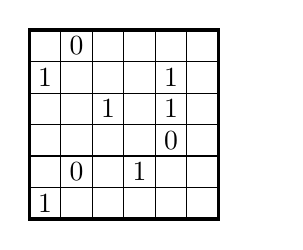
\begin{tikzpicture}[scale=0.4]
  % grid outer
  \draw[line width=1.2pt] (0,0) rectangle (6,6);

  % thin grid lines
  \foreach \i in {1,...,5}{
    \draw[line width=0.4pt] (\i,0) -- (\i,6);
    \draw[line width=0.4pt] (0,\i) -- (6,\i);
  }


  %---- ESEMPIO DI SUDOKU ----
  % riga 1
  \node[] at (0.5,0.5) {1};
  \node[] at (3.5,1.5) {1};
  \node[] at (4.5,2.5) {0};
  \node[] at (4.5,3.5) {1};
  
  \node[] at (1.5,1.5) {0};
  \node[] at (1.5,5.5) {0};
  \node[] at (0.5,4.5) {1};
  \node[] at (2.5,3.5) {1};
  \node[] at (4.5,4.5) {1};

    \node[] at (7.5,0.5) {}; % spostare il taku
  %\node[givennode, color=blue, fill=cyan!30] at (6.5,0.5) {1};

\end{tikzpicture}
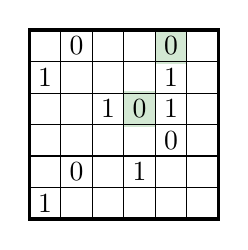
\begin{tikzpicture}[scale=0.4]
  % grid outer
  \draw[line width=1.2pt] (0,0) rectangle (6,6);

  % thin grid lines
  \foreach \i in {1,...,5}{
    \draw[line width=0.4pt] (\i,0) -- (\i,6);
    \draw[line width=0.4pt] (0,\i) -- (6,\i);
  }


  %---- ESEMPIO DI SUDOKU ----
  % riga 1
  \node[] at (0.5,0.5) {1};
  \node[] at (3.5,1.5) {1};
  \node[] at (4.5,2.5) {0};
  \node[] at (4.5,3.5) {1};
  \node[] at (1.5,1.5) {0};
  \node[] at (1.5,5.5) {0};
  \node[] at (0.5,4.5) {1};
  \node[] at (2.5,3.5) {1};
  \node[] at (4.5,4.5) {1};

  \node[color=black, fill=ForestGreen!20] at (4.5,5.5) {0};
  \node[color=black, fill=ForestGreen!20] at (3.5,3.5) {0};
  \draw[line width=1.2pt] (0,0) rectangle (6,6);
    \foreach \i in {1,...,5}{
    \draw[line width=0.4pt] (\i,0) -- (\i,6);
    \draw[line width=0.4pt] (0,\i) -- (6,\i);
  }
\end{tikzpicture}
\\
{\footnotesize
\textit{Es. Takuzu $6x6$, incompleto (sx) e con alcuni inserimenti (dx)}}
\end{center}

    
    \begin{osservazioni2}
    \underline{\textbf{Nota.}}\\
    \textit{Per semplicità e senza perdita di generalità, si assuma che allegando $\phi_=$ tramite and logico alla formula $\phi_{takuzu}$ proposta si includano le tutte le proprietà dell'uguale, così da permettere se necessario l'uso del \textbf{predicato} $=(\ \cdot\ ,\ \cdot\ )\ \subseteq \ Dominio\times Dominio$}. È possibile approfittare del risultato dell'esercizio precedente.
    \end{osservazioni2}

    




    
    %% INDEX
    \addcontentsline{toc}{subsection}{Esercizio 33.} 
    %%
    
    %\item \textbf{\textcolor{ForestGreen}{Esercizio 33.} \textcolor{blue}{(***)}}\\ 
    %Si completi il precedente esercizio formalizzando le proprietà dell'uguaglianza per il predicato $=(x,y)$. 
    
    
    
    
\end{itemize}
\vfill
\noindent\makebox[\linewidth]{\rule{\linewidth}{0.4pt}}
\end{document}